\section{R2CC Overview}

Figure~\ref{fig:architecture} summarizes how R2CC handles network failures during collective communication. R2CC is implemented as a drop-in extension of NCCL with RDMA support, the most widely deployed CCL for ML training and inference. When an inter-node failure occurs, R2CC transforms the CCL from fail-stop to fail-operational through three key components:

\smallskip\noindent\whitecircled{1}~\textbf{Fault detection and localization.} When a connection error surfaces during a collective (e.g., an immediate QP error, RDMA retry exhaustion), R2CC intercepts it and turns it into a recoverable CCL-managed event, then quickly localizes the fault to the affected side (local, remote, or bilateral). The localization result then drives live migration onto a backup connection (\S\ref{sec:design-mig}) and failure-aware scheduling (\S\ref{sec:single-failure}).

\smallskip\noindent\whitecircled{2}~\textbf{Live migration (HotRepair).} R2CC then migrates the ongoing collective onto a pre-established backup RDMA connection. Over the out-of-band (OOB) path, the two endpoints reconcile a replay boundary using NCCL protocol semantics rather than transport state alone (\S\ref{sec:design-mig}). This keeps replay correct even for CCL low latency protocol variants. Only the unreconciled suffix is retransmitted on the backup connection.

\begin{figure}
    \centering
    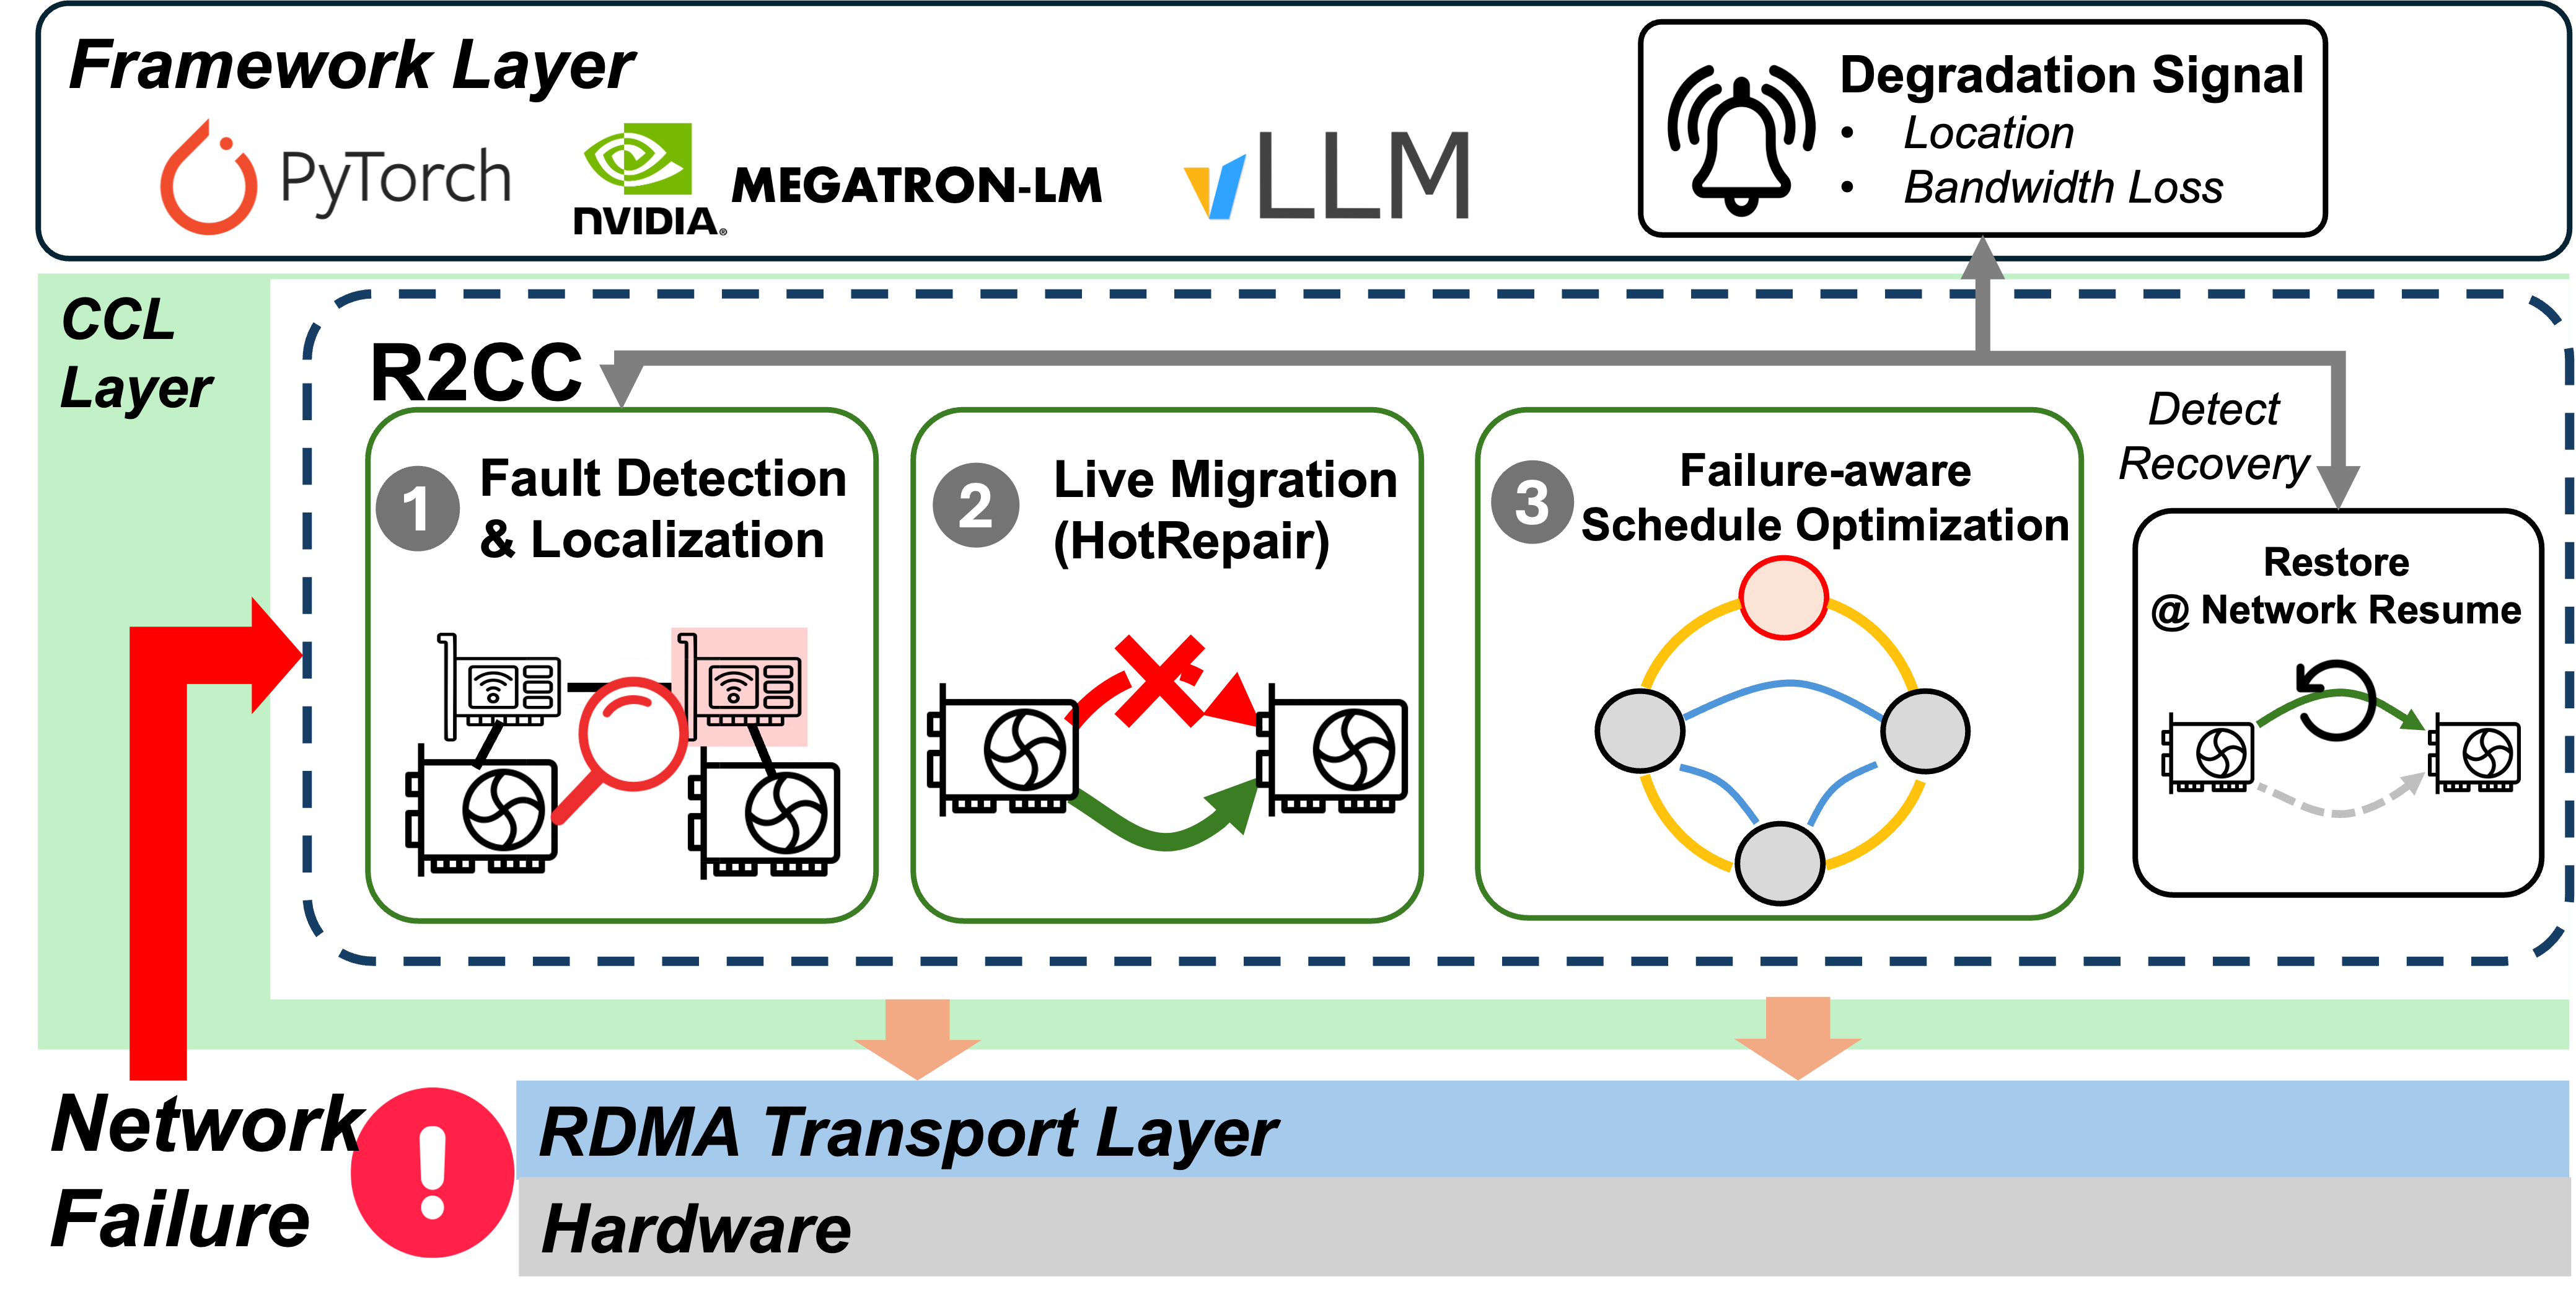
\includegraphics[width=1\columnwidth]{figs/new-overview.png}
    \vspace{-15pt}
    \tightcaption{\textbf{R2CC Overview.}}
    \label{fig:architecture}
    \vspace{-2mm}
\end{figure}

\smallskip\noindent\whitecircled{3}~\textbf{Failure-aware collective schedule optimization.}
HotRepair preserves correctness, but it does not, by itself, adapt the collective to the degraded heterogeneous topology. \textbf{R2CC-Balance} is the general optimization: it redistributes traffic from the failed NIC across surviving paths (e.g., PCIe forwarding or NVLink PXN\footnote{NVIDIA PXN~\cite{nccl-pxn} routes inter-server GPU traffic through intermediate GPUs as proxies.}) without changing the collective pattern, and applies broadly across collectives and P2P communication. For throughput-bound AllReduce on large messages, \textbf{R2CC-AllReduce} adds a specialized optimization on top of R2CC-Balance: it modifies the standard ring schedule to reduce data sent to and from the impaired server, further improving performance under degraded connectivity.

\smallskip\noindent\textbf{Degradation signaling and restore.}
As soon as a fault is localized, R2CC reports the degradation status to the framework, so the upper layer has both more policy choices and more time to act than it would under a later crash or abort. It can choose whether to continue running, run to its next safe boundary and then act, shrink, or restart. In the background, R2CC periodically probes the affected path. When the path becomes usable again, R2CC restores the original route, removes the corresponding scheduling adaptation, and updates the degradation signal.

\subsection{Challenges and Key Ideas}

\textbf{C1: Error visibility in an ongoing collective.} Hot repair must identify and pinpoint failures mid-collective before NCCL's default crash-on-error behavior triggers. In practice, NIC failures surface only as generic connection errors: the network stack cannot tell which endpoint actually failed, which creates \textit{asymmetric error visibility} that can leave peers waiting on a dead connection.

\textit{Key Idea:} R2CC introduces \textit{bilateral failure awareness} over a bootstrap network, combined with \textit{probe-based RDMA fault localization}, to rapidly locate the faulty endpoint. When a link between servers A and B fails, R2CC immediately notifies both sides over the out-of-band notification path to eliminate half-open states where one endpoint continues waiting on a dead connection, then triangulates the fault via three-point probing from a third peer in the same communicator.

\smallskip\noindent\textbf{C2: Lossless live migration over alternative links.} Even once the faulty NIC is known, NCCL's tight GPU--NIC binding prevents an ongoing collective from switching to an alternative path. Migration must also be lossless: the backup connection has to resume the collective without dropping or duplicating any in-flight chunk, under both throughput-oriented and low-latency CCL protocols.

\textit{Key Idea:} To break NCCL's GPU–NIC binding, R2CC pre-establishes idle backup connections to neighboring servers at initialization. These idle backup connections enable R2CC to reconcile a protocol-aware replay boundary with the peer and resume the collective on the backup connection without reinitializing NCCL.

\smallskip\noindent\textbf{C3: Online collective bandwidth optimization with single or multiple failures.} Network failures transform the cluster into a heterogeneous topology. Naively redirecting all traffic to a single backup NIC (i.e., basic HotRepair) often leads to congestion and bottlenecks. While solver-based schedule synthesis can find optimal routing, its high computational latency makes it unsuitable for real-time recovery. The primary challenge lies in rapidly generating failure-aware schedules that maximize bandwidth utilization within a degraded network.

\textit{Key Idea:} R2CC-Balance treats NICs as a unified resource pool, redistributing traffic through topology-aware heuristics. R2CC-AllReduce adapts the standard collective algorithm by proportionally balancing data loads according to degraded bandwidth. To address complex concurrent failures, R2CC generalizes these mechanisms through topology-aware logical re-ranking and recursive R2CC-AllReduce scheduling, maintaining high throughput across increasingly degraded topologies.
